%%%%%%%%%%%%%%%%%%%%%%%%%%%%%%%%%%%%%%%%%%%%%%%%%%%
%% P3: Phenomenology of Particle Physics                         
%%
%% Author:  André Rubbia                   		 
%%
%% Figure 2.5 The number of decays as a function of time in the three-element decay chain.
%%
%% This work is licensed under the Creative Commons Attribution 4.0 International License. 
%% To view a copy of this license, visit http://creativecommons.org/licenses/by/4.0/ or 
%% send a letter to Creative Commons, PO Box 1866, Mountain View, CA 94042, USA.
%%
%%%%%%%%%%%%%%%%%%%%%%%%%%%%%%%%%%%%%%%%%%%%%%%%%%%

\documentclass[a4paper,10pt]{article}

\usepackage[T1]{fontenc}
\usepackage[utf8]{inputenc}
\usepackage{lmodern}
\usepackage[labelfont=bf]{caption}
\usepackage{upgreek}
\usepackage{amssymb}
\usepackage{amsmath}

\usepackage{tikz}
\usepackage{pgfplots}
\pgfplotsset{compat=1.17}
\usepgfplotslibrary{ternary}
\usepgfplotslibrary{fillbetween}
\usepgfplotslibrary{external}

\def\d{\mathrm{d}}

\begin{document}

%%%%%%%%%%%%%%%   FIGURE  %%%%%%%%%%%%%%%%%%%%%%%%%%%%%%
\begin{figure}[htb]
\begin{center}
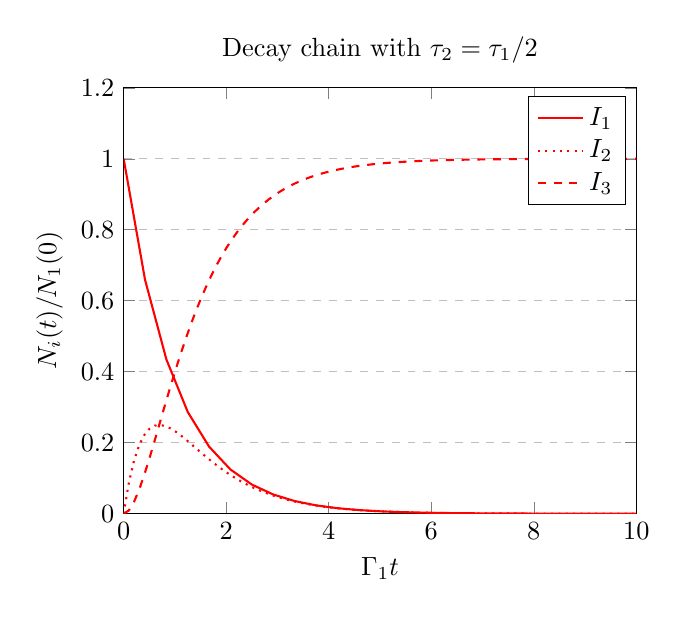
\begin{tikzpicture}[scale=0.95]
\begin{axis}[
    title={Decay chain with $\tau_2 = \tau_1/2$},
    xlabel={$\Gamma_1 t$},
    ylabel={$N_i(t)/N_1(0)$},
    xmin=0, xmax=10,
    ymin=0, ymax=1.2,
    ymajorgrids=true,
    grid style=dashed,
]
 \addplot[domain=0:10,thick, color=red] {exp{-x}};
 \addplot[domain=0:10,thick, dotted,color=red,samples=100] {(exp{-x}-exp{-2*x})};
 \addplot[domain=0:10,thick, dashed,color=red,samples=100] {1+exp{-2*x}-2*exp{-x})};
     \legend{$I_1$, $I_2$, $I_3$}
\end{axis}
\end{tikzpicture}
\hspace{5mm}
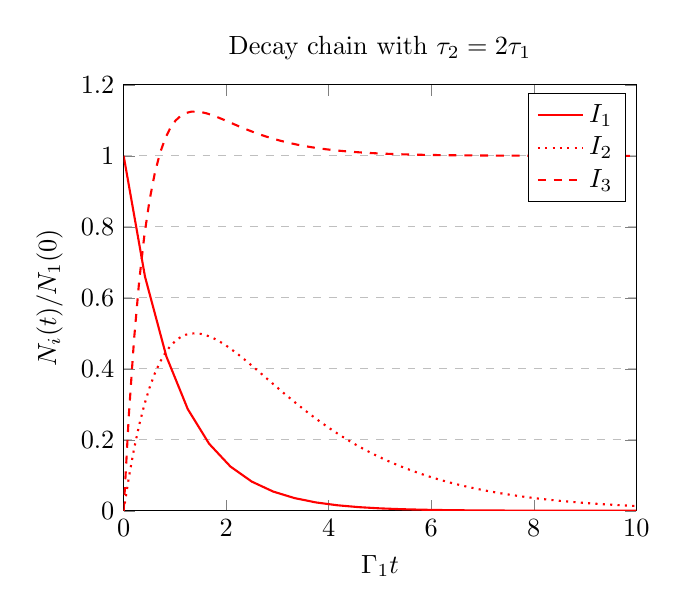
\begin{tikzpicture}[scale=0.95]
\begin{axis}[
    title={Decay chain with $\tau_2 = 2\tau_1$},
    xlabel={$\Gamma_1 t$},
    ylabel={$N_i(t)/N_1(0)$},
    xmin=0, xmax=10,
    ymin=0, ymax=1.2,
    ymajorgrids=true,
    grid style=dashed,
]
 \addplot[domain=0:10,thick, color=red] {exp{-x}};
 \addplot[domain=0:10,thick, dotted,color=red,samples=100] {-2*(exp{-x}-exp{-0.5*x})};
 \addplot[domain=0:10,thick, dashed,color=red,samples=100] {1-2*exp{-2*x}+exp{-x})};
     \legend{$I_1$, $I_2$, $I_3$}
\end{axis}
\end{tikzpicture}
\caption{The number of decays as a function of time in the three-element decay chain
$\protect I_1\stackrel{\tau_1}{\longrightarrow}
I_2 \stackrel{\tau_2}{\longrightarrow} I_3(\text{stable})$; (left) $\tau_2 = \tau_1/2$; (right)
$\tau_2 = 2\tau_1$.}
\end{center}
\end{figure}
%%%%%%%%%%%%%%%   END FIGURE  %%%%%%%%%%%%%%%%%%%%%%%%%%%%%%
%

\end{document}
